\chapter{Object Reconstruction}
\label{chap:objects}

In this chapter the physics objects necessary to be able to perform searches with \Pgt leptons
in the final state, and how they are reconstructed in \ac{CMS}, will be discussed. The 
descriptions correspond to the algorithms as used during Run 2. Where there are differences
between the algorithms used in Run 1 and Run 2 this will be discussed at the end
of the relevant section. Section \ref{sec:objects_pv} discusses the algorithms
used to reconstruct charged tracks in the inner tracker, with section \ref{sec:objects_ele}
describing how these tracks are combined with \ac{ECAL} energy deposits to reconstruct electrons.
In section \ref{sec:objects_muo} the combination of charged tracks in the inner tracker with
hits in the muon chambers to form reconstructed muons will be discussed. Section \ref{sec:objects_pf}
describes the \ac{PF} algorithm, which uses information from all subdetectors in \ac{CMS} to reconstruct
all stable particles, which is of particular importance for the reconstruction of jets, missing transverse
energy and hadronic taus as discussed in sections \ref{sec:objects_jets}, \ref{sec:objects_met} and \ref{sec:objects_tau} 
respectively.

\section{Tracks and vertices}
\label{sec:objects_pv}
To reconstruct the trajectories of charged particles, and therefore
their momenta and positions, from the hits these particles leave in the 
inner tracker, dedicated algorithms are required. In \ac{CMS} the
\ac{CTF} algorithm is used. This algorithm performs four steps:
\begin{itemize}
\setlength{\itemsep}{-\baselineskip}
\item Initial estimates of the parameters of the trajectory are given by track seeds, providing track candidates found using hits in 2 or 3 layers of the inner tracker
\item The track seeds are extrapolated using a Kalman filter \cite{trk-kf}, which extrapolates the seeding trajectories along the expected flight path of a charged particle 
and adds additional matched hits it finds in the tracker layers to the track.
\item After the extrapolation has reached the final tracker layers, the Kalman filter is run again, now with the full set of hits that have been found in the previous step.
This provides the best estimate of the track parameters
\item Tracks that fail a specified set of quality criteria are rejected
\end{itemize}

These four steps are repeated six times. After each iteration
the hits associated with reconstructed tracks are removed, and the settings
of the algorithm updated, so as to be able to reconstruct as many
tracks as possible. The tracking efficiency for muons and pions was measured in p--p
collisions at $\sqrt{s} = 7$ TeV and found to be $ > 98.5\%$ for tracks
with \pT $ > 500 $ MeV and $ > 99 \%$ for tracks with \pT $ > 2 $ GeV \cite{cms-trk-7tev}.

%The tracking software at CMS is commonly referred to as the Combinatorial Track Finder (CTF), which is an adaptation of the combinatorial Kalman filter [29–31], which in turn is an extension of the Kalman filter [32] to allow pattern recognition and track fitting to occur in the same frame- work. The collection of reconstructed tracks is produced by multiple passes (iterations) of the CTF track reconstruction sequence, in a process called iterative tracking.
%Kalman filter : In its linear form the Kal- ,nan filter is the optimal recursive estimator of the state vector of a (discrete) linear dynamic system. In such a system the evolution of the state vector is described by a linear transformation plus a random disturbance w, which is the process noise

The reconstructed tracks are used to determine the positions of all interaction
vertices in the event. Primary vertices are reconstructed by clustering
tracks that appear to have originated from the same vertex, then fitting 
for the position of the vertex using the associated tracks. The tracks 
are clustered using the \ac{DA} algorithm \cite{vtx-da}, which identifies
the most probable vertex candidates and assigns tracks to them. Vertex
candidates with at least two associated tracks are fitted using an adaptive
vertex fitter \cite{vtx-adaptivefit} to obtain the best estimate
of the vertex position as well as an indicator for the success of the fit.
Each track is assigned a weight $w_i$ between 0 and 1 which reflects the probability
that it belongs to the vertex it is associated with. If the track is consistent
with the vertex position the weight will be closer to 1, if not the weight 
will be smaller. Using this the number of degrees of freedom in the fit
can be defined as
\begin{equation}\label{eqn:pv_ndof}
n_{\text{dof}} = -3 + 2 \Sigma_{i=1}^{Ntracks}w_i,
\end{equation}
which is strongly correlated with the number of tracks arising from the interaction region
and can therefore be used to select genuine interactions. For the analysis
presented in chapter \ref{chap:hhh}, which uses data collected during Run 1, to select the primary vertex, 
this variable
was required to be greater than 4, in addition to requirements on the distance between
the vertex and the nominal interaction point ($\Delta z < 24$ cm and $\Delta x-y < 2$ cm). 
The primary vertex was then taken as the vertex passing these quality criteria that 
had the largest scalar sum \pT of associated tracks. For the Run 2 analyses presented
later the quality requirements were removed and the primary vertex, the vertex
of the hard scattering process, is simply taken as the reconstructed vertex with
largest scalar sum \pT of associated tracks.
The resolution of the z--coordinate of the primary vertex was measured in
collisions at $\sqrt{s}=7$ TeV and depends strongly on the number of tracks
associated with the vertex, as figure \ref{fig:objects_tracks_pvres} shows.

\begin{figure}
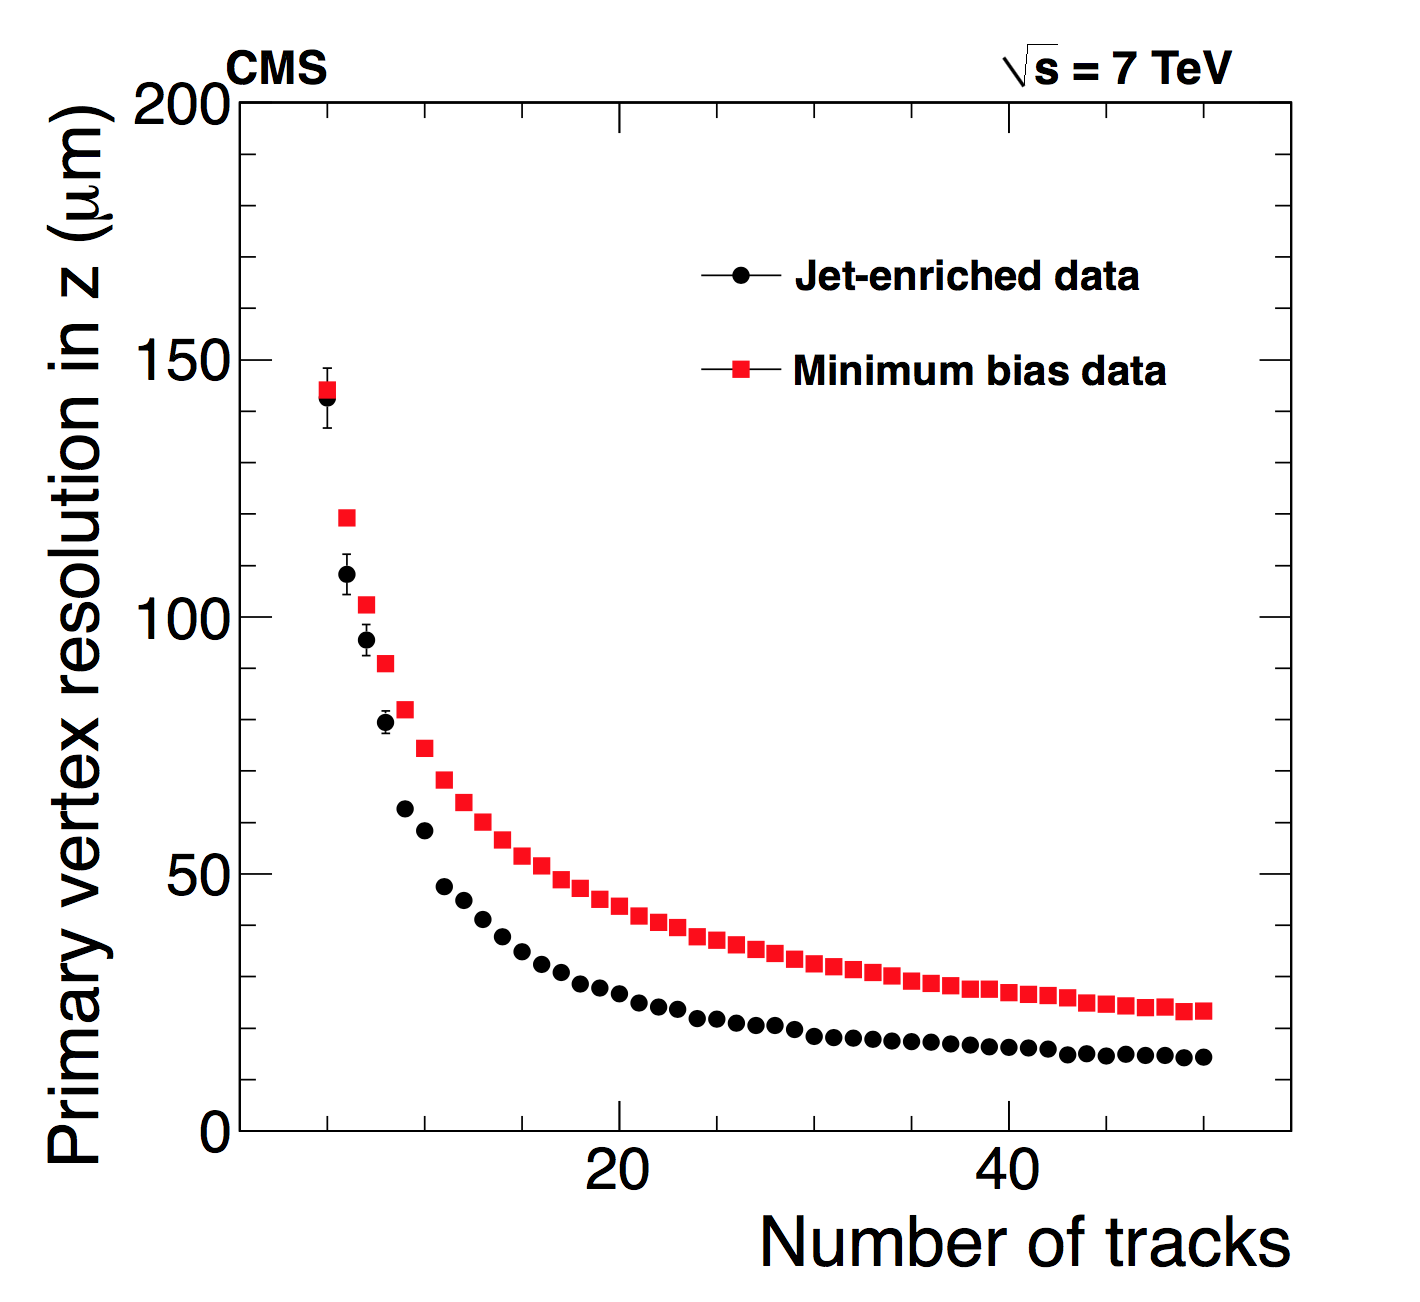
\includegraphics[width=0.5\textwidth]{./Objects/Plots/PrimaryVertexRes.png}
\caption{Resolution of the z--coordinate of reconstructed primary vertices
as a function of the number of tracks associated with the vertex, 
for minimum--bias events in red and for
events with many jets in black. The resolution improves
with larger numbers of tracks \cite{cms-trk-algos}.}
\label{fig:objects_tracks_pvres}
\end{figure}

\section{Electrons}
\label{sec:objects_ele}
Electrons are reconstructed by combining tracks reconstructed
in the inner tracker with energy deposits in the \ac{ECAL} \cite{cms-elereco-run1}.
A standalone electron reconstruction algorithm \cite{cms-elereco-run1} complements the \ac{PF} approach
described in section \ref{sec:objects_pf}. Because electrons lose on average 33-86\% of
their energy by radiating photons before the \ac{ECAL} is reached, depending on the thickness of
the intervening material. To accurately reconstruct the energy of the electron it is
important to catch the energies of photons, which are spread in the $\phi$ direction
due to the magnetic field. Therefore \textit{supercluster} algorithms are needed to perform
the clustering. In this approach the clustering
is done by defining a seed crystal as the one containg the most energy deposited
in a region being considered and having a certain minimum transverse energy.
In the barrel arrays of $5\times 1$ crystals in $\eta \times \phi$ are then added
to the cluster, stepping sideways in both directions in $\phi$, if this
array contains a minimum energy deposit. These clusters are grouped into 
superclusters if each distinct cluster has a seed array with a minimum energy deposit.
In the endcaps the clusters combined into superclusters are arrays of $5\times 5$ crystals,
merged into superclusters within a range in $\eta$ of $\pm 0.07$ and a range in $\phi$ of $\pm 0.3$ rad.

Because the electrons radiate bremsstrahlung photons in the tracker, the
change in electron track curvature is large. The reconstruction of these
tracks using the \ac{CTF} is compromised as a result of this, and 
therefore a dedicated tracking algorithm is used. For high \pT electrons
the best efficiency is reached by using an \ac{ECAL}-based track seeding
algorithm which extrapolates the position and energy of the supercluster
to the first layers of the tracker to determine rough areas to look for
tracker seeds in. Once the seeds have been determined they are extrapolated
and smoothed using the \ac{GSF} \cite{trk-gsf} instead of the Kalman Filter, which 
approximates the non-Gaussian energy loss in each layer by the combination of 
Gaussian distributions rather than the single Gaussian used in the Kalman filter.

%Once the hits are collected, a GSF fit is performed to estimate the track parameters. The energy loss in each layer is approximated by a mixture of Gaussian distributions. A weight is at- tributed to each Gaussian distribution that describes the associated probability. Two estimates of track properties are usually exploited at each measurement point that correspond either to the weighted mean of all the components, or to their most probable value (mode).

To be identified as an electron, a particle has to be reconstructed as
an electron by the \ac{PF} algorithm, and must in addition pass
more advanced identification criteria based on some of the variables used in the
standalone electron reconstruction, which provide separation power from backgrounds
such as photon conversions, jets misidentified as electrons, or electrons from b- and c-quark
decays. Both cut--based and MVA--based algorithms are available. For the selection of electrons in 
the analyses presented in later chapters these MVA--based algorithms are usually used, 
with exceptions for the loose identification criteria required for veto-electrons. 
The variables used to train the electron identification BDT are:

\begin{itemize}
\setlength{\itemsep}{-\baselineskip}
\item Cluster shape variables $\sigma_{i\eta,i\eta}$ and $\sigma_{i\phi,i\phi}$, with $i\eta$ and $i\phi$ the integer
label of the $\eta$ and $\phi$ calorimeter cell. The circularity =  $1 -\frac{E1\times5}{E5\times5}$, with
$E1\times5$ and $E5\times5$ the energies in a $1\times5$ and a $5\times5$ grid around the super cluster seed,
respectively. Shape variable R9 = $\frac{E3\times3}{E_{SC}}$, with $E3\times3$ the energy in a $3\times3$ grid
of cells around the super cluster seed and $E_{SC}$ the raw energy of the super cluster.
\item The number of valid hits in the track fit, the $\chi^2$ of the track fit and the $\chi^2$ of the GSFTrack fit
\item The number of GSFtrack hits, the number of expected missing inner hits and the result of the conversion vertex fit
\item The distance $\Delta \eta$ and $\Delta \phi$ between the reconstructed super cluster and the associated track at the position of the primary vertex, and the distance in $\eta$ between the super cluster and the track at the calorimeter surface.
\item H/E, the ratio of the hadronic energy over the electromagnetic energy in the super cluster and E/P, the ratio of the super cluster energy over the momentum of the track associated with the electron
\item The ratio of the energy of the electron cluster and the momentum of the associated track, evaluated at the electron cluster,
 and $1/E_e - 1/P_e$, with $E_e$ the energy of the electron candidate and $P_e$ its momentum.
\end{itemize}

\subsection{Isolation}
The identification requirements discussed up to now reduce the backgrounds 
from misidentified electrons, but do not eliminate them completely. If jets are
misidentified as electrons, or an electron resulting from a heavy--flavour 
decay is identified, the electron is not isolated. Therefore requirements
on the electron isolation can reduce these backgrounds even further.
Different isolation definitions are used in \ac{CMS}, for the analyses presented
in later chapters a combined isolation variable is defined as:
\begin{equation}\label{eqn:electron_reliso
I_{\text{rel}} = \frac{\Sigma p_{\text{T}}(\text{charged}) + \mathrm{max}(\Sigma E_{\text{T}}(\text{neutral}) + \Sigma E_{\text{T}}(\text{photon}) - \Delta\beta \Sigma E_{\text{T}}(\text{PU}),0)}{P_{T}^{e}},
\end{equation}
Where the \pT and \ET sums are taken within a cone in $\eta - \phi$ around the direction
of the electron, $\Delta R = 0.4$ during Run 1 and $\Delta R = 0.3$ during Run 2.
The sum over \pT$^{\text{charged}}$ corresponds to the \pT of all charged \ac{PF} 
hadrons associated with the primary vertex and within 
Where \pT$^{\text{charged}}$ corresponds to the \pT of all charged \ac{PF} hadrons
associated with the primary vertex

Where $P_{T}(\text{charged})$ corresponds to the $P_{T}$ of all charged hadronic candidates,
$E_{T}(\text{photon, neutral})$ to the transverse energy of all photon and neutral hadron candidates, and $\Delta \beta$ is the energy
esitmate of neutral particles due to pileup, which is taken to be 0.5.


\section{Muons}
\label{sec:objects_muo}

\section{\acl{PF}}
\label{sec:objects_pf}
All stable particles are reconstructed and identified using the \ac{PF} algorithm \cite{cms-pf-2009,cms-pf-2010-commfirst,cms-pf-2010-2}, which
combines the information from all of the different subdetectors of \ac{CMS}. This makes
the identification of particles, and determination of position and momentum, as precise
as possible. All of these particles are then used to build for example jets, \MET and hadronically
decaying taus.

The \ac{PF} algorithm starts from charged particle tracks measured
by the inner tracker, muon tracks measured in the muon system, and 
energy deposits in the calorimeters. These energy deposits are combined
using a clustering algorithm, so that stable neutral particles can be identified,
separated from charged hadrons, and electrons and all Bremsstrahlung photons
can be reconstructed. Clustering is performed separately in the \ac{ECAL} barrel,
\ac{ECAL} endcaps, first and second \ac{PS} layers, \ac{HCAL} barrel and \ac{HCAL} endcaps, with no 
clustering employed in the \ac{HF}.
%And to aid energy measurement of charged hadrons for which
%tracks were low quality, or high pT
The clustering algorithm used for \ac{PF} starts from \textit{cluster seeds},
calorimeter cells with local energy maxima. Topological clusters are built by 
merging neighbouring cells into the cluster, provided that the cells
being merged in contain a certain minimum energy.
The threshold is 800 MeV in the \ac{HCAL} and two standard deviations above the
expected noise level in the \ac{ECAL}, meaning 80 MeV in the barrel and up 
to 300 MeV in the endcaps. Cell energies can be shared between multiple
\ac{PF} clusters, depending on the distance between a cell and the centre of the cluster.

Any given particle will usually give rise to multiple \ac{PF}
elements in the different subdetectors. To provide full reconstruction
of each particle, and avoid double counting,  the next step in the
\ac{PF} algorithm is to link the different elements. This is
achieved by defining a distance parameter between any two \ac{PF} elements
in the event, which quantifies the link quality. Directly and indirectly
linked elements are considered as input blocks to the reconstruction and
identification algorithm. Links between charged tracks and calorimeter
clusters are established by extrapolating the track from its last measured
tracker hit to the \ac{PS} layers, the \ac{ECAL} and the \ac{HCAL}. %in ECAL to expected maximum of a 
%typical longitudinal electron shower profile and in the HCAL at a depth correspnding to one interaction
%length.
If the extrapolated track position is within the boundaries of the cluster, plus the size
of one cell in each direction to account for gaps between cells and multiple scattering, the
track is said to be linked to the calorimeter cluster. The distance is taken as the distance $\Delta R$ 
between the position of the cluster and the position of the track. Tangents to tracks are also extrapolated
to the ECAL from the track--tracker layer interaction points, and clusters can be 
linked to the track as a possible Bremsstrahlung photon if the extrapolated tangent
position is within the boundaries of the cluster.
Links between calorimeter clusters are made when the cluster position in the
more granular calorimeter is within the cluster of the less granular calorimeter,
with the link distance again defined as the $\Delta R$ between two cluster positions.
To determine links between charged tracks in the inner tracker and a muon track
in the muon system, a global fit between the two tracks is performed, where the link
is accepted if requirements on the maximum $\chi^2$ of this fit are met. This
$\chi^2$ also determines the distance parameter.

For each block, particles are identified following a sequence
of tests. First, if there is a link between a tracker track and a muon system track,
a particle flow muon is identified if the combined tracker and muon system
momentum is compatible with the tracker-only momentum. %within three standard deviations
The muon track is removed from the block before the next step of the algorithm.

Secondly, tracks are refitted with the \ac{GSF}, the compatibility
of the track with the already linked \ac{ECAL} clusters is assessed using
\ac{BDTs} which take several variables into account. If the candidate
passes, it is identified as a particle flow electron and the track and
\ac{ECAL} clusters are removed from the block.

Following this, remaining tracks lead to charged hadrons. The track is
given the momentum from the track fit, assuming the mass of a charged pion. If
the energy measured in the calorimeters is compatible with the momentum assigned
to the track, within uncertainties, as charged hadron is identified and the
momentum redefined by fitting the tracker and calorimeter measurements. If
the energy of the calorimeter clusters linked to the track is significantly larger than the
charged particle momentum from the track fit, additional overlapping neutral particles
are identified. If the difference between tracker momentum and calorimeter
energies is larger than the total energy registered in associated \ac{ECAL} clusters,
a particle flow photon with energy equal to the total \ac{ECAL} energy is created.
Any remaining momentum difference is assigned to a particle flow neutral hadron. If the momentum
difference is smaller than the energy registered in associated \ac{ECAL} clusters 
only a particle flow photon is created. %Justified by fact that
%in jets 25% of the energy is carried by photons while neutral hadrons
%leave only 3% of the jet energy in the ECAL. This fraction is reduced by one order of magnitued
%for taus for which decays to final states with neutral hadrons are Cabbibo suppressed to a branching ratio of 
%about a percent.

Finally, any remaining \ac{ECAL} clusters not linked to a track give
rise to particle flow photons, with any \ac{HCAL} clusters
not linked to tracks giving rise to particle flow neutral hadrons.



\section{Jets and b-tagging}
\label{sec:objects_jets}

\subsection{Jet energy corrections}
\label{sec:objects_jets_jec}

\section{Missing energy}
\label{sec:objects_met}

\subsection{Recoil corrections}
\label{sec:objects_met_recoilcorr}

\section{Hadronic taus}
\label{sec:objects_tau}
Taus are unstable particles and they decay before reaching the detector. In 17.4 \% of 
cases they decay to muons and neutrinos, with an additional 17.8 \% decaying to electrons
plus neutrinos. The remaining 64.8 \% decay hadronically. Hadronically decaying
taus are characterised by narrow jets containing either one or three charged
particles ($\pi^{\pm}, K^{\pm}$) and 0,1, or two neutral pions. An overview
of the most common possible decay modes is given in table \ref{tab:hadronic_tau_decays}

\begin{table}[htp]
\begin{center}
\caption{Summary of hadronic tau decay modes, indicating the branching fraction, and intermediate resonances where relevant \cite{pdg-2014}.}
\begin{tabular}{@{}lll@{}}
%\toprule
\textbf{Decay mode} & \textbf{Resonance} &\textbf{Branching fraction [\%]}\\
\midrule
\Ptaupm $\rightarrow$ h$^{\pm}$\Pnut & & 11.5\%\\
\Ptaupm $\rightarrow$ h$^{\pm}$\Ppizero\Pnut& $\rho$(770) & 26.0\% \\
\Ptaupm $\rightarrow$ h$^{\pm}$\Ppizero\Ppizero\Pnut & a$_{1}$(1260) & 9.5\% \\
\Ptaupm $\rightarrow$ h$^{\pm}$h$^{\mp}$h$^{\pm}$\Pnut & a$_{1}$(1260) & 9.8\% \\
\Ptaupm $\rightarrow$ h$^{\pm}$h$^{\mp}$h$^{\pm}$\Ppizero\Pnut & & 4.8\%\\
Other modes with hadrons & & 3.2\% \\
\midrule
Total & & 64.8\% \\
%\bottomrule
\end{tabular}
\label{tab:hadronic_tau_decays}
\end{center}
\end{table}

\subsection{Identification}
\label{sec:objects_tau_id}
Hadronic tau decays are reconstructed using the \texttt{hadrons plus strips} (HPS) algorithm~\cite{cms-tau-run1,cms-tau-2015}, 
which is seeded by jets clustered from \ac{PF} candidates, using the anti-\kT algorithm with a distance parameter $\Delta R = 0.4$. 
As table \ref{tab:hadronic_tau_decays}
shows, 60\% of hadronic tau decays contain at least one \Ppizero in the final state. There is a high
probability that photons from $\Ppizero \rightarrow \Pphoton \Pphoton$ decays convert to
\APelectron \Pelectron pairs in the tracker volume, which are bent in the magnetic field and 
therefore cause showers dispersed in the $\phi$ direction in the \ac{ECAL}. Therefore, to 
reconstruct the energy deposits \Ppizero candidates leave in the ECAL, 
the photon and electron constituents of the jet that seeds the $\tau_{h}$ reconstruction are clustered into strips.
The \Pe or \Pphoton with highest \pT that is not yet included in a strip is used to build a new strip.
The $\eta$ and $\phi$ of this candidate determine the initial position of the strip, the next highest \pT \Pe or \Pphoton  
within an $\eta \times \phi$ window centered on the strip location is added to the strip and the position is 
recomputed as the energy-weighted average of the electron/photon constituents in the strip.
This procedure is repeated until there are no more electrons or photons with \pT $> 0.5$~GeV  within the 
strip window. The $\Delta \eta$ and $\Delta \phi$ of the strip are varied based on the \pT or \ET to 
be added to the strip and on the energy the strip already has, as
\begin{equation}\label{eqn:dynamicstrip}
\begin{split}
&\Delta \eta  = f(p_{\text{T}}^{\Pe/\Pphoton}) + f(p_{\text{T}}^{\text{strip}}) \\
&\Delta \phi  = g(p_{\text{T}}^{\Pe/\Pphoton}) + g(p_{\text{T}}^{\text{strip}})\\
\end{split}
\end{equation}
Where \pT$^{\Pe/\Pphoton}$ is the transverse momentum of the candidate to be added to the strip
and \pT$^{\text{strip}}$ is the transverse momentum of the strip before merging a new candidate in.\\
In addition, the strip size is bounded as $0.05 < \Delta\eta < 0.15$, $0.05 < \Delta\phi < 0.3$ \cite{cms-tau-2015}.

The functions $f(p_{\text{T}})$ and $g(p_{\text{T}})$ are defined as:
\begin{equation}\label{eqn:dynamicstripfg}
\begin{split}
&f(p_{\text{T}}) = 0.2\cdot p_{\text{T}}^{-0.66} \text{ and } \\
&g(p_{\text{T}}) = 0.35\cdot p_{\text{T}}^{-0.71}.\\
\end{split}
\end{equation}
If the $\Sigma$ \pT of the strip is at least 2.5~GeV, it is considered as a \Ppizero candidate.
To reconstruct hadronic taus, charged particles and strips are combined into different signatures which are said to be
compatible with a certain decay mode if the selection listed below is satisfied. The charged particles
and strips are required to be within the signal cone $R_{\text{signal}} = \frac{3.0}{p_{\text{T}}[GeV]}$, always
required to be $0.05 < R_{\text{sig}} < 0.1$.
If a candidate satisfies more than one of the hypotheses, the one that maximises the \pT is retained.\\

The decay modes considered for reconstructing hadronic taus are:
\begin{itemize}
\setlength{\itemsep}{-\baselineskip}
\item \textbf{One prong + 0 \Ppizero :} One charged particle, no strips.
\item \textbf{One prong + 1 \Ppizero :} One charged particle + one strip with mass $ 0.3 < m_{\Pgt} < 1.3 \sqrt{p_{\text{T}}/100}$~GeV. For momenta
less than 100 GeV, the upper limit is fixed to 1.3 GeV, and for momenta larger than 1044 GeV the upper limit on $m_{\Pgt}$ is fixed to 4.2 GeV.
\item \textbf{One prong + 2 \Ppizero :} One charged particle + two strips. The $\Pgt$ mass should be $0.4 < m_{\Pgt} < 1.2\sqrt{p_{\text{T}}/100}$~GeV. For momenta
less than 100 GeV, the upper limit is fixed to 1.2 GeV and for momenta larger than 1111 GeV the upper limit on $m_{\Pgt}$ is fixed to 4.0 GeV.
\item \textbf{Three prong + 0 \Ppizero: } Three charged particles with mass $0.8 < m_{\tau} < 1.5$~GeV. The tracks are required to originate 
within $\Delta z<0.4$~cm of the same vertex, and their total charge is required to be $\pm 1$.
\end{itemize}

\subsection{Isolation and discrimination against light leptons}
\label{sec:objects_tau_iso}
Requiring the reconstructed $\Pgt_{h}$ to be isolated reduces the jet $\rightarrow\Pgt_{h}$ fake rate. The isolation
can be defined using a cut--based discriminator using the isolation sum,
\begin{equation}\label{eqn:cutbased_iso}
I_{\Pgt} = \Sigma p_{\text{T}}^{\text{charged}}(d_Z < 0.2\text{ cm }) + \text{max}(0,\Sigma p_{\text{T}}^{\Pphoton} - \Delta \beta \Sigma p_{\text{T}}^{\text{charged}} (d_Z > 0.2 \text{ cm }) ),
\end{equation}
where the first term denotes the sum of the transverse momenta of all charged particles not part
of the identified hadronic tau,  with \pT $> 0.5$ GeV within a cone $\Delta R = 0.5$ centred around the 
direction of the hadronic tau, with charged particle tracks required to be compatible with having
originated from the $\Pgt_{h}$ production vertex within $d_Z < 0.2$ cm. The second term denotes the sum
of the transverse momenta of photons with \pT $ > 0.5$ GeV within a cone $\Delta R = 0.5$ centred around the direction
of the hadronic tau. The effect of pile--up on this term is accounted for by subtracting the sum of the momenta of charged
particles with \pT $ > 0.5$ GeV, within a cone of $\Delta R = 0.8$ around the direction of the hadronic tau and
tracks not compatible with having originated from the production vertex of the hadronic tau, multiplied by
a $\Delta \beta$ factor of 0.2.

In addition to the isolation sum, a selection on the sum of transverse momenta
of electrons and photons included in strips but which are located outside of the signal cone,
\begin{equation}\label{eqn:ptouter_iso}
p_{\text{T}}^{\text{strip, outer}} = \Sigma p_{\text{T}}^{\Pe/\Pphoton}(\Delta R > R_{\text{sig}}) < 0.10\cdot p_{\text{T}}^{\Pgt}.
\end{equation}
An  MVA $\tau_{h}$ isolation discriminator combines isolation variables with $\tau$ lifetime information into a BDT to discriminate between $\tau_{h}$ decays and quark and gluon jets.
The variables used as input are:\\
\begin{itemize}
\setlength{\itemsep}{-\baselineskip}
\item The charged-and neutral-particle isolation sums
\item The reconstructed $\tau_{h}$ decay mode
\item The transverse impact parameter $d_{xy}$ of the leading track of the $\tau_{h}$ candidate with the vertex, and its significance $d_{xy}/\sigma_{d_{xy}}$, and its sign (the projection of the impact parameter vector on the $\tau_h$ direction)
\item The 3-dimensional impact parameter $d_{xyz}$ of the leading track, and it significance
\item The distance between the $\tau$ production and decay vertices, its significance, and information about whether a decay vertex has successfully been reconstructed for a given candidate.
\item $p_{\text{T}}$ and $\eta$ of the $\tau_{h}$ candidate
\item $\Delta \beta$ corrected isolation (as equation \ref{eqn:cutbased_iso}
\item The sum of transverse momenta of electrons and photons included in strips but located outside of the signal cone (equation \ref{eqn:ptouter_iso})
\item The $\chi^2$ value of the fit for the leading track of the $\tau_{h}$ candidate
\item The ratio of the total electromagnetic energy to the total energy within the $\tau_h$ signal cone.
\item The total number of signal and isolation photons with $p_{\text{T}} > 0.5$~GeV
\item The $p_{\text{T}}$ weighted $\Delta R$ of photons within signal cone and the isolation annulus
\item The $p_{\text{T}}$ weighted $\Delta \eta$ and $\Delta \phi$ of photons in strips outside of the signal cone.
\end{itemize}

Figure \ref{fig:tau_iso_efficiency} compares the \Pgt identification efficiency with the
jet$\rightarrow \Pgt_{h}$ fake rate for different working points of the
MVA isolation discriminator, as well as the cut--based isolation discriminator based
on isolation sum and $p_{\text{T}}^{\text{strip,outer}}$. The MVA--based 
discriminator has better performance than the cut-based discriminator alone.

\begin{figure}
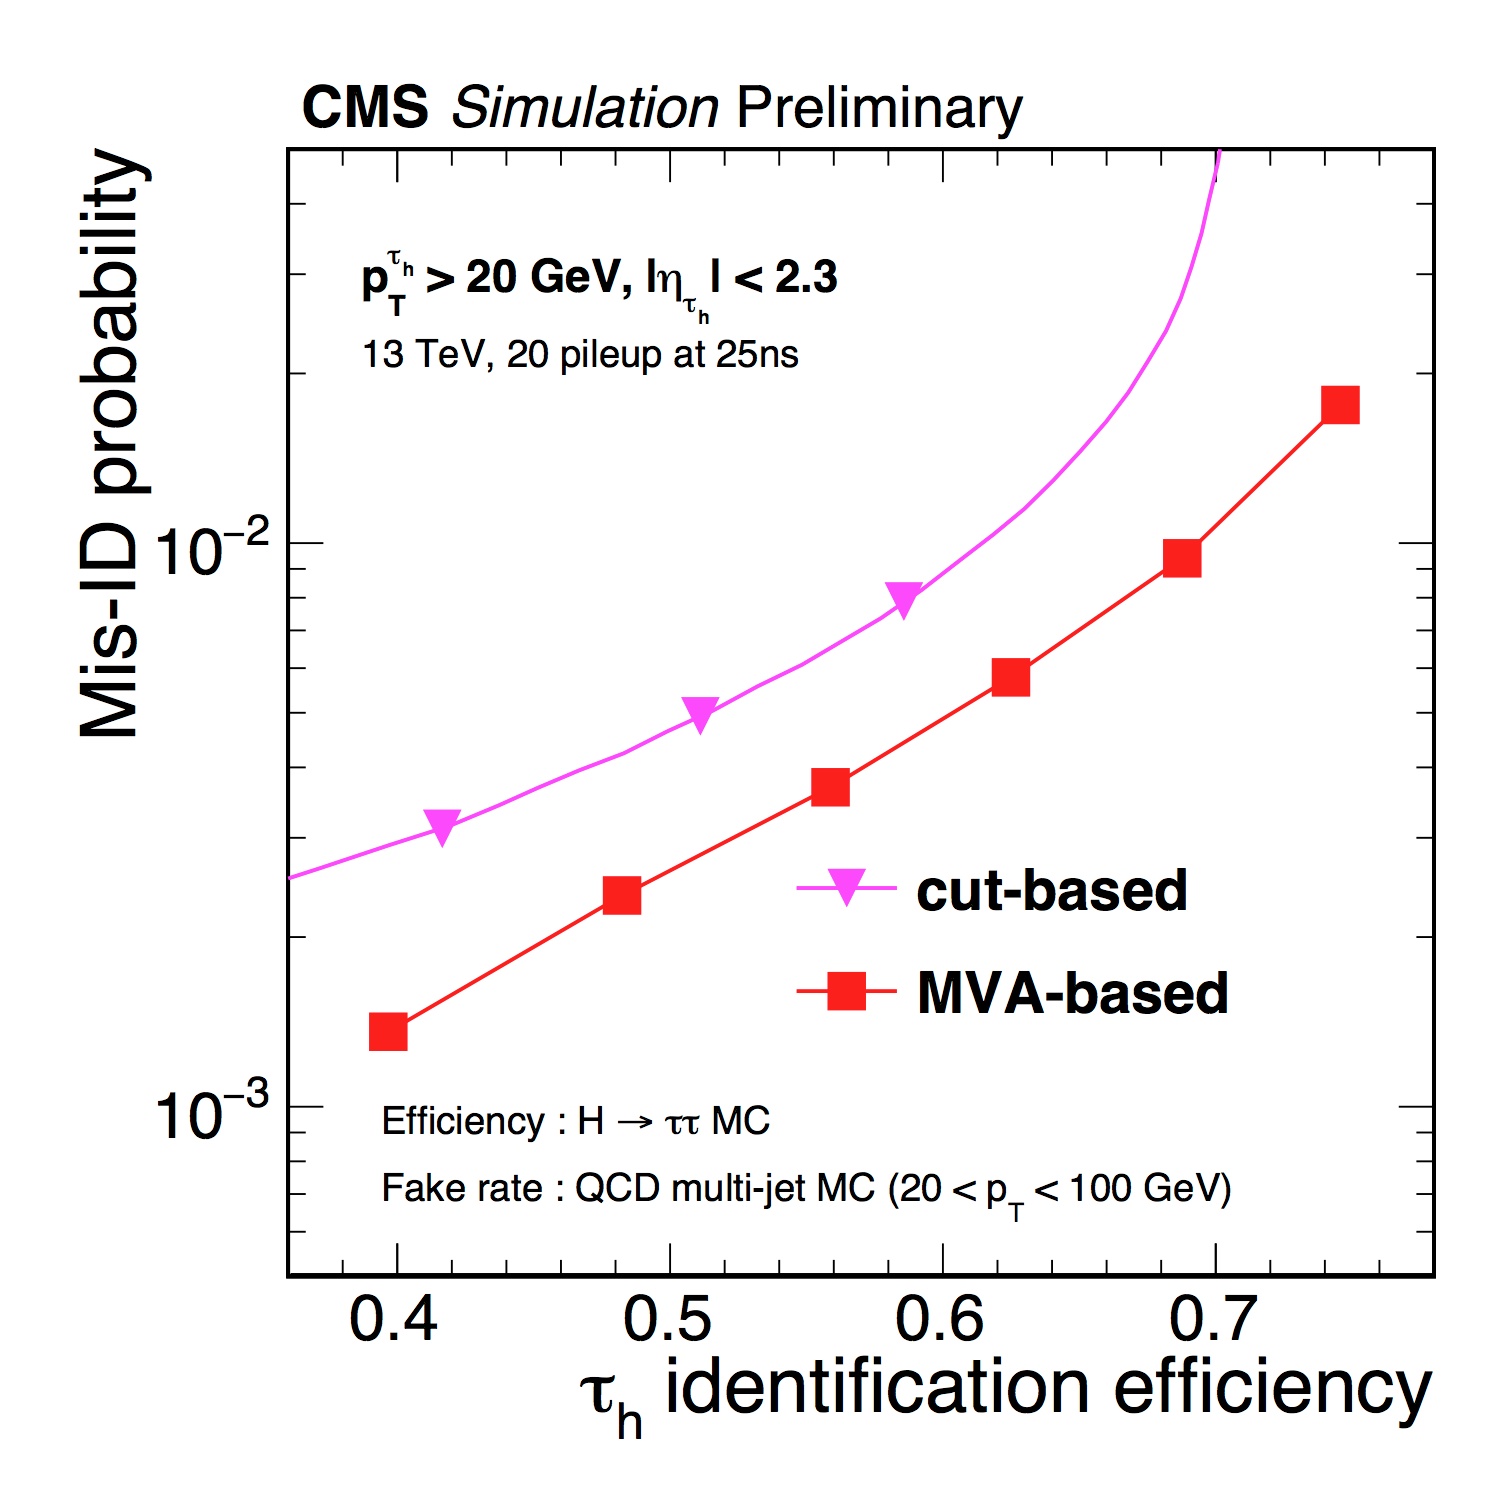
\includegraphics[width=0.7\textwidth]{./Objects/Plots/TauIsolationPlot.png}
\caption{jet$\rightarrow \Pgt_{h}$ fake rate versus $\Pgt_{h}$ identification efficiency for \htotautau events,
comparing the MVA-based discriminator in red with the cut-based isolation discriminator in pink. Tighter working points
give lower hadronic tau identification efficiencies and lower fake rates. The MVA-based discriminator
has a lower fake rate than the cut-based discrminator for the same $\Pgt_{h}$ identification efficiency \cite{cms-tau-2015}.}
\label{fig:tau_iso_efficiency}
\end{figure}

In order to reduce the $Pe\rightarrow\Pgt_h$ and $\Pgm\rightarrow\Pgt_h$ fake rate, 
anti-electron and anti--muon discriminators are used. 
The anti--electron discriminator is a BDT-based discriminator with the following input variables:
\begin{itemize}
\setlength{\itemsep}{-\baselineskip}
\item \pT, $\eta$ of the $\Pgt_{h}$ candidate
\item \pT, $\eta$, $\sigma_{p_{\text{T}}}/p_{\text{T}}$ of the \ac{GSF} track
\item Distance in $\eta$ and $\phi$ of the \ac{GSF} track to the nearest boundary between \ac{ECAL} modules.
\item Electromagnetic energy fraction $E_{\text{ECAL}}/(E_{\text{ECAL}}+E_{\text{HCAL}})$
\item Ratio of \ac{ECAL} and \ac{HCAL} energy fractions relative to the momentum of the leading charged track
\item The \pT weighted RMS distances in $\eta$ and $\phi$ between the photons in any strip and the leading 
charged track (calculated separately for photons inside and outside the $\Pgt$ signal cone)
\item The fraction of $\Pgt_{h}$ energy carried by photons (calculated separately for photons inside and outside the $\Pgt_h$ signal cone)
\item $(p_{in} - p_{out})/p_{in}$
\item The number of photons in any of the strips associated with the $\Pgt_h$ candidate, calculated separately for photons inside and outside the $\Pgt_h$ signal cone
\item The ratio between the total \ac{ECAL} energy and inner track momentum
\item The ratio of energies of bremsstrahlung photons measured in the \ac{ECAL} and the tracker
\item The visible mass of the $\Pgt_h$ candidate, for photons and charged particles within the $\Pgt_h$ signal cone
\item $\chi^2/Ndof$ of the GSF track fit
\item $N_{hits}^{GSF}-N_{hits}^{KF}/N_{hits}^{GSF}+N_{hits}^{KF}$, With $N_{hits}^{GSF}$ the number of hits associated with the track in the \ac{GSF} track reconstruction algorithm, and
similarly $N_{hits}^{KF}$ for the \ac{KF} track reconstruction algorithm.
\end{itemize}

Five working points are provided, ranging from very loose to very tight.

The anti--muon discriminator is a cut-based discriminant, for which two working points are provided:\\
\begin{itemize}
\setlength{\itemsep}{-\baselineskip}
\item \textbf{Loose:} The $\tau_h$ candidate is vetoed by this discriminator if track segments are found in at least two muon stations within a cone of $\Delta R = 0.3$ of the $\Pgt_h$ direction, or when the sum of the electromagnetic and hadronic energy ($E_{\text{ECAL}}+E_{\text{HCAL}}$) is $<0.2\cdot p_{\text{leading track}}$.
Otherwise it passes the discriminator
\item \textbf{Tight:} The $\Pgt_h$ candidate passes this working point if it passes the loose working point and no hits are present within a cone of $\Delta R=0.3$ of the $\Pgt_h$ direction in the \ac{CSCs},\ac{RPCs} and \ac{DT} in the two outermost muon stations.
\end{itemize}

\subsection{Differences between Run 1 and Run 2}
\label{sec:objects_taus_diff}
Broadly speaking the algorithm used for hadronic tau reconstruction during Run 1
was similar to the Run 2 algorithm described earlier in this section \cite{cms-tau-run1}. However, during
Run 1 strips were reconstructed using a fixed size of $0.05 \times 0.20$ in $\eta \times \phi$.
The dynamic size used in Run 2 was introduced to mitigate the effects of secondary particles
with low \pT and multiple \APelectron\Pelectron conversions, resulting in particles ending up outside of 
the strip window and making the hadronic tau seem less isolated than it actually is.
In addition, the anti--electron discriminator MVA was trained with fewer input variables and its performance
was therefore not as good as the Run 2 version.


